\documentclass[../../main.tex]{subfiles}
\begin{document}

\begin{flushright}
  \footnotesize\textit{【自動文字起こし・要確認】}
\end{flushright}

% Source: handwritten.pdf 第4問．
{\bf [解]}
$f(x)=x^2-2$，$g(x)=2x^2+ax-1$とおく．$g(0)=-1<0$から，$g$の2次係数が正なので
$g(x)=0$は必ず2異実根を持ち，
\begin{align}x=\dfrac{-a\pm\sqrt{a^2+8}}{4}
\end{align}
である．これを$\alpha,\beta$ $(\alpha<\beta)$とおく．

\subparagraph{(i) $-\dfrac{3\sqrt{2}}{2}<a<\dfrac{3\sqrt{2}}{2}$の時}
$-\sqrt{2}\leqq\alpha<\beta\leqq\sqrt{2}$となるから，
$x\leqq\alpha$，$\beta\leqq x$に分けて考える．
\begin{figure}[H]
  \centering
  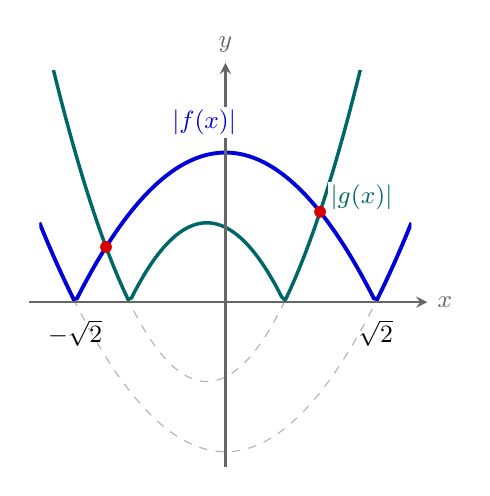
\begin{tikzpicture}[x=1.35cm,y=.95cm,>=stealth,
    every node/.style={font=\small}]
    % 配置例として a=0.7 を選ぶ。
    \begin{scope}
      \clip (-1.75,-2.1) rectangle (1.75,3.1);
      \draw[dashed,gray!60,domain=-1.75:1.75,samples=90]
      plot (\x,{\x*\x-2});
      \draw[dashed,gray!60,domain=-1.75:1.75,samples=90]
      plot (\x,{2*\x*\x+.7*\x-1});
      \draw[blue!85!black,line width=1.4pt,domain=-1.75:1.75,samples=110]
      plot (\x,{abs(\x*\x-2)});
      \draw[teal!80!black,line width=1.25pt,domain=-1.75:1.75,samples=110]
      plot (\x,{abs(2*\x*\x+.7*\x-1)});
    \end{scope}
    \draw[->,thick,gray!80!black] (-1.85,0)--(1.9,0) node[right] {$x$};
    \draw[->,thick,gray!80!black] (0,-2.2)--(0,3.2) node[above] {$y$};
    \foreach \sgn in {-1,1} {
      \pgfmathsetmacro{\t}{(-.7+\sgn*sqrt(36.49))/6}
      \node[circle, fill=red!85!black, inner sep=1.5pt] at (\t,{abs(\t*\t-2)}) {};
    }
    \node[blue!85!black,fill=white,inner sep=1pt] at (-.2,2.4) {$|f(x)|$};
    \node[teal!80!black,fill=white,inner sep=1pt] at (1.28,1.4) {$|g(x)|$};
    \node[below=3pt] at (-1.414,0) {$-\sqrt{2}$};
    \node[below=3pt] at (1.414,0) {$\sqrt{2}$};
  \end{tikzpicture}
  \caption{$a=0.7$での$f,g$（灰色破線）と$|f|,|g|$の配置}
\end{figure}
\subparagraph{(a) $|x|\geqq\sqrt{2}$の時}
\begin{align}
  f(x)=g(x)\ \Longleftrightarrow\ x^2+ax+1=0
  \ \Longleftrightarrow\ x=\dfrac{-a\pm\sqrt{a^2-4}}{2}.
\end{align}
ここで$|a|\leqq\dfrac{3\sqrt{2}}{2}$から
\begin{align}
  \dfrac{-a-\sqrt{a^2-4}}{2}>-\sqrt{2},\qquad
  \dfrac{-a+\sqrt{a^2-4}}{2}<\sqrt{2}
\end{align}
なので，$|x|\geqq\sqrt{2}$の区域に解なし．

\subparagraph{(b) $\alpha<x<\beta$の時}
$|f(x)|=|g(x)|\Longleftrightarrow f(x)=g(x)$であり，(a)からグラフの対応は下図のようになっているので，
\begin{align}
  |a|<2\text{の時 }0\text{つ},\qquad
  |a|=2\text{の時 }1\text{つ},\qquad
  |a|>2\text{の時 }2\text{つ}.
\end{align}
\begin{figure}[H]
  \centering
  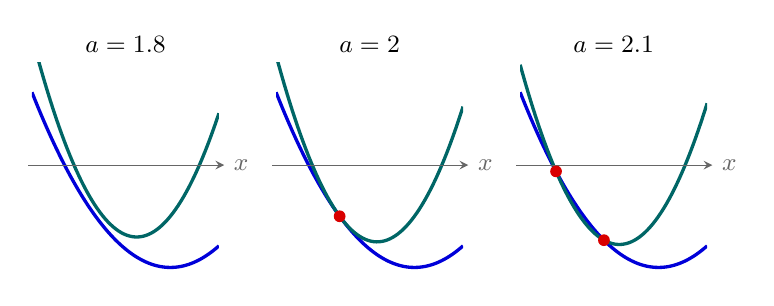
\begin{tikzpicture}[x=.95cm,y=.65cm,>=stealth,
    every node/.style={font=\small}]
    \foreach \v/\dx/\lab in {1.8/0/{$a=1.8$},2/3.1/{$a=2$},2.1/6.2/{$a=2.1$}} {
      \begin{scope}[xshift=\dx cm]
        \begin{scope}
          \clip (-1.85,-2.2) rectangle (.65,2.0);
          \draw[blue!85!black,line width=1.2pt,domain=-1.85:.65,samples=70]
          plot (\x,{\x*\x-2});
          \draw[teal!80!black,line width=1.2pt,domain=-1.85:.65,samples=70]
          plot (\x,{2*\x*\x+\v*\x-1});
        \end{scope}
        \draw[->,gray!80!black] (-1.9,0)--(.72,0) node[right] {$x$};
        \node[above] at (-.6,2.0) {\lab};
      \end{scope}
    }
    \begin{scope}[xshift=3.1cm]
      \node[circle, fill=red!85!black, inner sep=1.5pt] at (-1,-1) {};
    \end{scope}
    \begin{scope}[xshift=6.2cm]
      \foreach \sgn in {-1,1} {
        \pgfmathsetmacro{\t}{(-2.1+\sgn*sqrt(.41))/2}
        \node[circle, fill=red!85!black, inner sep=1.5pt] at (\t,{\t*\t-2}) {};
      }
    \end{scope}
  \end{tikzpicture}
  \caption{$\alpha<x<\beta$における$f$（青）と$g$（緑）の共有点数の変化}
\end{figure}

\subparagraph{(ii) $\dfrac{3\sqrt{2}}{2}<a$の時}
$\alpha<-\sqrt{2}<\beta<\sqrt{2}$となるから，2次係数に注意してグラフは下図のようになり，4個ある．
\begin{figure}[H]
  \centering
  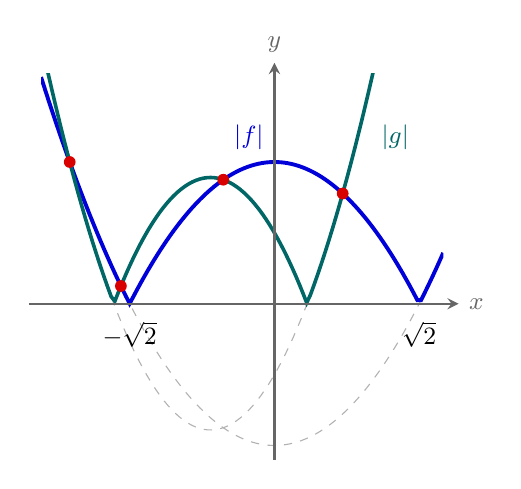
\begin{tikzpicture}[x=1.3cm,y=.9cm,>=stealth,
    every node/.style={font=\small}]
    % a=2.5 では x=-2,-3/2,-1/2,2/3 が共有点の x 座標。
    \begin{scope}
      \clip (-2.28,-2.1) rectangle (1.65,3.25);
      \draw[dashed,gray!60,domain=-2.28:1.65,samples=100]
      plot (\x,{\x*\x-2});
      \draw[dashed,gray!60,domain=-2.28:1.65,samples=100]
      plot (\x,{2*\x*\x+2.5*\x-1});
      \draw[blue!85!black,line width=1.4pt,domain=-2.28:1.65,samples=110]
      plot (\x,{abs(\x*\x-2)});
      \draw[teal!80!black,line width=1.3pt,domain=-2.28:1.65,samples=110]
      plot (\x,{abs(2*\x*\x+2.5*\x-1)});
    \end{scope}
    \draw[->,thick,gray!80!black] (-2.4,0)--(1.8,0) node[right] {$x$};
    \draw[->,thick,gray!80!black] (0,-2.2)--(0,3.4) node[above] {$y$};
    \foreach \t in {-2,-1.5,-.5,.666667}
    \node[circle, fill=red!85!black, inner sep=1.5pt] at (\t,{abs(\t*\t-2)}) {};
    \node[below=3pt] at (-1.414,0) {$-\sqrt{2}$};
    \node[below=3pt] at (1.414,0) {$\sqrt{2}$};
    \node[blue!85!black,fill=white,inner sep=1pt] at (-.25,2.35) {$|f|$};
    \node[teal!80!black,fill=white,inner sep=1pt] at (1.18,2.35) {$|g|$};
  \end{tikzpicture}
  \caption{$a=2.5>3\sqrt{2}/2$のときの4つの共有点}
\end{figure}

\subparagraph{(iii) $a=\dfrac{3\sqrt{2}}{2}$の時}
$g(x)=2x^2+\dfrac{3\sqrt{2}}{2}x-1$で，グラフは下図で解は3つ．
\begin{figure}[H]
  \centering
  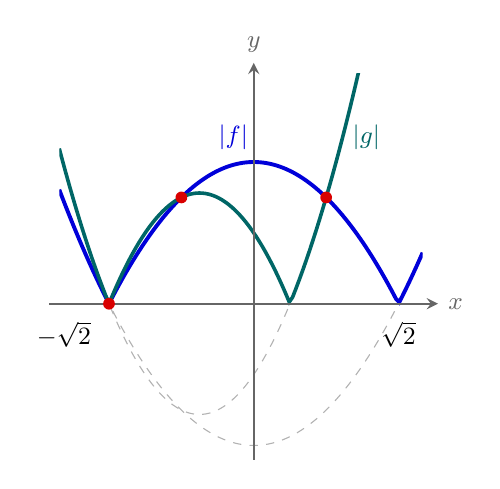
\begin{tikzpicture}[x=1.3cm,y=.9cm,>=stealth,
    every node/.style={font=\small}]
    \begin{scope}
      \clip (-1.9,-2.1) rectangle (1.65,3.25);
      \draw[dashed,gray!60,domain=-1.9:1.65,samples=100]
      plot (\x,{\x*\x-2});
      \draw[dashed,gray!60,domain=-1.9:1.65,samples=100]
      plot (\x,{2*\x*\x+1.5*sqrt(2)*\x-1});
      \draw[blue!85!black,line width=1.4pt,domain=-1.9:1.65,samples=110]
      plot (\x,{abs(\x*\x-2)});
      \draw[teal!80!black,line width=1.3pt,domain=-1.9:1.65,samples=110]
      plot (\x,{abs(2*\x*\x+1.5*sqrt(2)*\x-1)});
    \end{scope}
    \draw[->,thick,gray!80!black] (-2,0)--(1.8,0) node[right] {$x$};
    \draw[->,thick,gray!80!black] (0,-2.2)--(0,3.4) node[above] {$y$};
    \foreach \t in {-1.414214,-.707107,.707107}
    \node[circle, fill=red!85!black, inner sep=1.5pt] at (\t,{abs(\t*\t-2)}) {};
    \node[below left=3pt] at (-1.414,0) {$-\sqrt{2}$};
    \node[below=3pt] at (1.414,0) {$\sqrt{2}$};
    \node[blue!85!black,fill=white,inner sep=1pt] at (-.2,2.35) {$|f|$};
    \node[teal!80!black,fill=white,inner sep=1pt] at (1.1,2.35) {$|g|$};
  \end{tikzpicture}
  \caption{$a=3\sqrt{2}/2$のときの3つの共有点}
\end{figure}
対称性から$a\leqq-\dfrac{3\sqrt{2}}{2}$についても同様だから，
\begin{align}
  \begin{cases}
    4\text{つ}&a<-\dfrac{3\sqrt{2}}{2},\quad-\dfrac{3\sqrt{2}}{2}<a<-\sqrt{2},\quad
    \sqrt{2}<a<\dfrac{3\sqrt{2}}{2},\quad\dfrac{3\sqrt{2}}{2}<a,\\
    3\text{つ}&a=\pm\dfrac{2\sqrt{2}}{3},\quad\pm2,\\
    2\text{つ}&-\sqrt{2}<a<\sqrt{2}.
  \end{cases}
\end{align}
% 上の最終分類は原稿通り．途中の |a|=2，a=3\sqrt{2}/2 の記述と一致しないので要確認．

\medskip\noindent{\bf [別解]}
\begin{align}
  |f(x)|=|g(x)|&\ \Longleftrightarrow\ 2x^2+ax-1=\pm(x^2-2)\\
  &\ \Longleftrightarrow\ a=\dfrac{-2x^2+1\pm(x^2-2)}{x}\quad(x=0\text{は解でない}),\\
  &\ \Longleftrightarrow\ a=-\left(x+\dfrac{1}{x}\right)\quad\text{又は}\quad
  a=-3x+\dfrac{3}{x}.
\end{align}
グラフから解は分かる．
\begin{figure}[H]
  \centering
  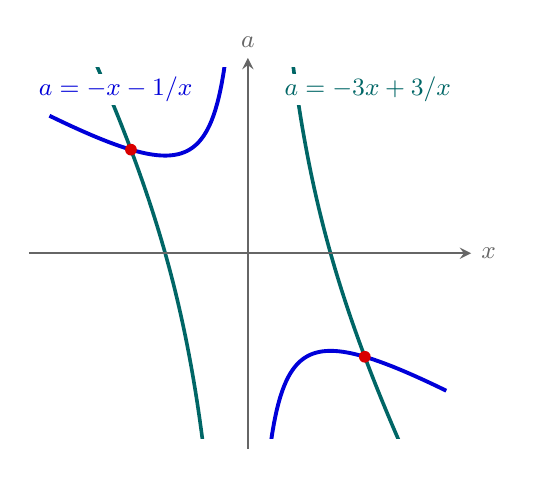
\begin{tikzpicture}[x=1.05cm,y=.62cm,>=stealth,
    every node/.style={font=\small}]
    \begin{scope}
      \clip (-2.5,-3.8) rectangle (2.5,3.8);
      \foreach \lo/\hi in {-2.4/-.22,.22/2.4} {
        \draw[blue!85!black,line width=1.4pt,domain=\lo:\hi,samples=90]
        plot (\x,{-\x-1/\x});
        \draw[teal!80!black,line width=1.3pt,domain=\lo:\hi,samples=90]
        plot (\x,{-3*\x+3/\x});
      }
    \end{scope}
    \draw[->,thick,gray!80!black] (-2.65,0)--(2.7,0) node[right] {$x$};
    \draw[->,thick,gray!80!black] (0,-4)--(0,4) node[above] {$a$};
    \foreach \sgn in {-1,1} {
      \pgfmathsetmacro{\t}{\sgn*sqrt(2)}
      \node[circle, fill=red!85!black, inner sep=1.5pt] at (\t,{-\t-1/\t}) {};
    }
    \node[blue!85!black,fill=white,inner sep=1pt] at (-1.6,3.35)
    {$a=-x-1/x$};
    \node[teal!80!black,fill=white,inner sep=1pt] at (1.45,3.35)
    {$a=-3x+3/x$};
  \end{tikzpicture}
  \caption{別解における$a=-x-1/x$，$a=-3x+3/x$のグラフ}
\end{figure}

\end{document}
